\documentclass{beamer}
\usetheme{Warsaw}

\usepackage{amsfonts} % math symobls
\usepackage{amsthm}
\usepackage[utf8]{inputenc}
\usepackage{polski}
\usepackage{graphics}
\usepackage{verbatim}
\usepackage{tikz}
\usetikzlibrary{arrows}
\usetikzlibrary{calc}

\newtheorem{tw}{Twierdzenie}
\newtheorem{lem}{Lemat}
\newtheorem{df}{Definicja}
\newtheorem{obs}{Obserwacja}  

\newcommand{\emp}[1]{\textcolor{blue}{\textit{#1}}}
\newcommand{\red}[1]{\textcolor{red}{#1}}
\newcommand{\tuple}[2]{\langle #1 , #2 \rangle}

\title{A Fully Dynamic Reachability Algorithm for Directed Graphs}
\subtitle{with an Almost Linear Update Time}
\author{Michał Karpiński}
\date{8 stycznia, 2013}

\begin{document}

\begin{frame}[plain]
  \titlepage
\end{frame}

\begin{frame}{Specyfika problemu (wersja statyczna)}
Dane: 

\begin{itemize}
\item graf skierowany $G$ oraz wierzchołki $u,v \in V(G)$
\end{itemize}

Wynik:

\begin{itemize}
\item Odpowiedź na pytanie: czy w $G$ istnieje ścieżka z $u$ do $v$?
\end{itemize}

\vspace{0.5cm}

\begin{center}
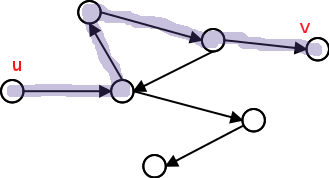
\includegraphics[scale=0.5]{Diagram1.png}
\end{center}

\end{frame}

\begin{frame}{Specyfika problemu (wersja dynamiczna)}

Różnica: graf $G$ zmienia się w czasie!


\vspace{0.5cm}

Cel: zbudowanie struktury danych wspierającej operacje:
\begin{itemize}
\item \emp{Update} - aktualizuje graf
\item \emp{Query} - odpowiada na pytanie o osiągalność
\end{itemize}
\end{frame}

\begin{frame}{Silnie spójne składowe (SSS)}

\begin{df}
{\bf Silnie spójna składowa} grafu skierowanego $G$ to taki maksymalny podgraf $H$, a jednocześnie jego spójna składowa, taka, że pomiędzy każdymi dwoma jej wierzchołkami istnieje ścieżka.
\end{df}

\begin{center}
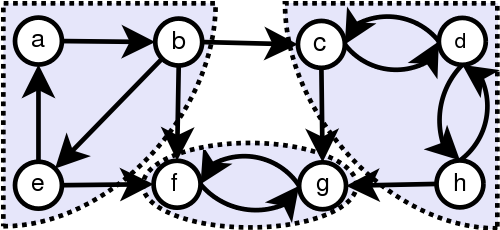
\includegraphics[scale=0.5]{Scc.png}
\end{center}

\end{frame}

\begin{frame}{Silnie spójne składowe (SSS)}
Problem: mając dany graf $G$, czy $u,v \in V(G)$ należą do tej samej silnie spójnej składowej?

\vspace{0.5cm}

\begin{itemize}
\item wersja statyczna - proste
\item wersja dynamiczna - zaraz się okaże :)
\end{itemize}

\vspace{0.5cm}

\begin{block}{Uwaga}
Struktura rozwiązująca problem dynamiczny SSS jest kluczem do utworzenia struktury rozwiązującej problem dynamiczny osiągalności w grafie skierowanym!
\end{block}

\end{frame}

\begin{frame}{Porządane procedury}

\begin{itemize}
\item \emp{Insert(E')} - tworzy nową \red{wersję grafu}, początkowo identyczną z poprzednią \red{wersją}, w której dodajemy zbiór krawędzi $E'$
\item \emp{Delete(E')} - usuwa zbiór krawędzi $E'$ ze \red{{\bf wszystkich} wersji grafu}
\item \emp{Query(u,v,i)} - sprawdza, czy $u$ i $v$ należą do wspólnego komponentu w $i$-tej wersji grafu
\end{itemize}

\end{frame}

\begin{frame}{Porządane procedury}
\begin{block}{Bardziej formalnie}
Algorytm zachowuje komponenty grafów $G_1,G_2 \cdots G_t$, gdzie $t$ jest liczbą operacji \emp{Insert} wykonaną do tej pory. Definiujemy $G_i=\tuple{V}{E_i}$ jako graf utworzony po $i$-tej operacji \emp{Insert}.
\end{block}

\begin{block}{Uproszczenie}
Zakładamy, że graf początkowy $G_0=\tuple{V}{E_0}$ jest grafem bez krawędzi, czyli $E_0 = \phi$. 
\end{block}
\end{frame}


%%% PIERWSZA PARTIA
\begin{frame}{Przykład}

\begin{columns}
\begin{column}<1->{0.25\textwidth}
\begin{center}$G_0$\end{center}
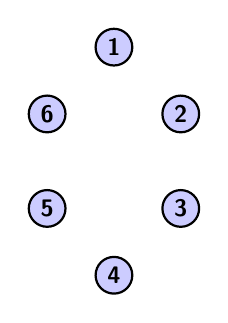
\begin{tikzpicture}[->,>=stealth',shorten >=1pt,auto,node distance=2cm,
  thick,main node/.style={circle,fill=blue!20,draw,font=\sffamily\Large\bfseries}]

  \node[main node,scale=0.6] (1) {1};
  \node[main node,scale=0.6] (2) [below right of=1] {2};
  \node[main node,scale=0.6] (3) [below of=2] {3};
  \node[main node,scale=0.6] (4) [below left of=3] {4};
  \node[main node,scale=0.6] (6) [below left of=1] {6};
  \node[main node,scale=0.6] (5) [below of=6] {5};
\end{tikzpicture}
\end{column}

\begin{column}<2->{0.25\textwidth}
\begin{center}$G_1$\end{center}
\begin{tikzpicture}[->,>=stealth',shorten >=1pt,auto,node distance=2cm,
  thick,main node/.style={circle,fill=blue!20,draw,font=\sffamily\Large\bfseries}]

  \fill<3->[fill=blue,fill opacity=0.4] ($(6.west)+(-0.25,0.4)$) -- ($(6.east)+(0.25,0.4)$) -- ($(5.east)+(0.25,-0.4)$) -- ($(5.west)+(-0.25,-0.4)$) -- cycle; 

  \node[main node,scale=0.6] (1) {1};
  \node[main node,scale=0.6] (2) [below right of=1] {2};
  \node[main node,scale=0.6] (3) [below of=2] {3};
  \node[main node,scale=0.6] (4) [below left of=3] {4};
  \node[main node,scale=0.6] (6) [below left of=1] {6};
  \node[main node,scale=0.6] (5) [below of=6] {5};

  \path
    (3) edge node [left] {} (4)
    (5) edge [bend left] node[left] {} (6)
    (6) edge [bend left] node[left] {} (5)
        edge node[right] {} (1);
\end{tikzpicture}
\end{column}

\begin{column}<4->{0.25\textwidth}
\begin{center}$G_2$\end{center}
\begin{tikzpicture}[->,>=stealth',shorten >=1pt,auto,node distance=2cm,
  thick,main node/.style={circle,fill=blue!20,draw,font=\sffamily\Large\bfseries}]

\fill<5->[fill=green,fill opacity=0.4] ($(6.west)+(-0.25,0.4)$) -- ($(6.east)+(0.25,0.4)$) -- ($(3.east)+(0.25,0.4)$) -- ($(3.east)+(0.25,-1.25)$) -- ($(5.west)+(-0.25,-1.25)$) -- cycle; 

  \node[main node,scale=0.6] (1) {1};
  \node[main node,scale=0.6] (2) [below right of=1] {2};
  \node[main node,scale=0.6] (3) [below of=2] {3};
  \node[main node,scale=0.6] (4) [below left of=3] {4};
  \node[main node,scale=0.6] (6) [below left of=1] {6};
  \node[main node,scale=0.6] (5) [below of=6] {5};

  \path
    (3) edge node [left] {} (4)
    (5) edge [bend left] node[left] {} (6)
        edge node [right] {} (3)
    (4) edge [bend right] node [left] {} (6)
    (6) edge [bend left] node[left] {} (5)
        edge node[right] {} (1);
\end{tikzpicture}
\end{column}

\begin{column}<6->{0.25\textwidth}
\begin{center}$G_3$\end{center}
\begin{tikzpicture}[->,>=stealth',shorten >=1pt,auto,node distance=2cm,
  thick,main node/.style={circle,fill=blue!20,draw,font=\sffamily\Large\bfseries}]

\fill<7->[fill=red,fill opacity=0.4] ($(6.west)+(-0.25,0.4)$) -- ($(2.east)+(0.25,0.4)$) -- ($(3.east)+(0.25,-1.20)$) -- ($(5.west)+(-0.25,-1.20)$) -- cycle;

  \node[main node,scale=0.6] (1) {1};
  \node[main node,scale=0.6] (2) [below right of=1] {2};
  \node[main node,scale=0.6] (3) [below of=2] {3};
  \node[main node,scale=0.6] (4) [below left of=3] {4};
  \node[main node,scale=0.6] (6) [below left of=1] {6};
  \node[main node,scale=0.6] (5) [below of=6] {5};

  \path
    (2) edge node {} (3)
    (3) edge node [left] {} (4)
    (5) edge [bend left] node[left] {} (6)
        edge node [right] {} (3)
    (4) edge [bend right] node [left] {} (6)
    (6) edge [bend left] node[left] {} (5)
        edge node[right] {} (1)
        edge node[right] {} (2);
\end{tikzpicture}
\end{column}
\end{columns}

\only<8>{\vspace{0.5cm}\begin{obs}
Każdy komponent z $G_i$ jest albo kompenentem z $G_{i-1}$, albo sumą pewnych komponentów z $G_{i-1}$.
\end{obs}}

\onslide<9->{\vspace{0.2cm}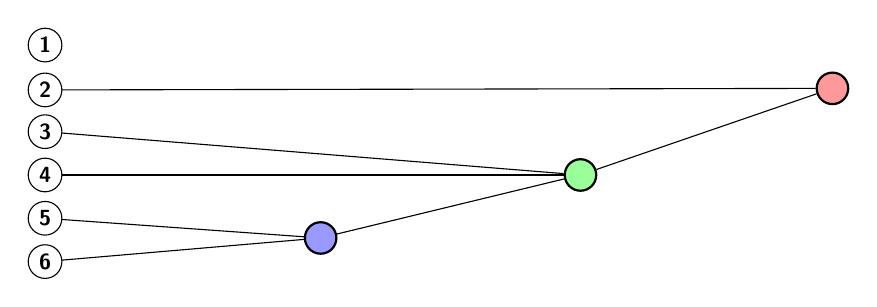
\begin{tikzpicture}[main node/.style={circle,fill=white!20,draw,font=\sffamily\Large\bfseries}]
  \node[thick,circle,fill=blue,fill opacity=0.4,minimum width=0.4cm,draw] (g1) at (3.5,-2.45) {};
  \node[thick,circle,fill=green,fill opacity=0.4,minimum width=0.4cm,draw] (g2) at (6.8,-1.65) {} edge (g1);
  \node[thick,circle,fill=red,fill opacity=0.4,minimum width=0.4cm,draw] (g3) at (10,-0.55) {} edge (g2);
  \node[main node,scale=0.55] (1) at (0,0) {1};
  \node[main node,scale=0.55] (2) at (0,-0.57) {2} edge (g3);
  \node[main node,scale=0.55] (3) at (0,-1.1) {3} edge (g2);
  \node[main node,scale=0.55] (4) at (0,-1.65) {4} edge (g2);
  \node[main node,scale=0.55] (5) at (0,-2.2) {5} edge (g1);
  \node[main node,scale=0.55] (6) at (0,-2.75) {6} edge (g1);

\end{tikzpicture}}

\end{frame}

\begin{frame}{Oko}
\end{frame}

\end{document}
